\documentclass[12pt]{article}
\usepackage[utf8]{inputenc}
\usepackage[english]{babel}
\usepackage{amsmath}
\usepackage{amssymb}

\usepackage[top=2.5cm, bottom=3cm, left=3.5cm, right=3.5cm, headheight=16pt]{geometry}
\parindent = 0cm				         
\parskip   = 8pt	%salto de linea

\usepackage{hyperref}
\hypersetup{
    colorlinks=true,
    linkcolor=blue,
    filecolor=magenta,      
    urlcolor=blue,
}

\usepackage{graphicx}
\graphicspath{ {images/} }

\title{Machine Learning Lecture Notes}
\author{by Andrew Ng}
\date{Transcripted by: Fernando García de la Cruz}

\begin{document}
\maketitle
\chapter{Week 1}
\section{What is Machine Learning?}
Two definitions of Machine Learning are offered. {\bf Arthur Samuel} described it as: {\bf ``the field of study that gives computers the ability to learn without being explicitly programmed."} This is an older, informal definition.

{\bf Tom Mitchell} provides a more modern definition: 
\begin{quote}
``A computer program is said to learn from experience E with respect to some class of tasks T and performance measure P, if its performance at tasks in T, as measured by P, improves with experience E."
\end{quote}
Example: playing checkers.

E = the experience of playing many games of checkers \\[1pt]
T = the task of playing checkers.\\[1pt]
P = the probability that the program will win the next game.

In general, any machine learning problem can be assigned to one of two broad classifications: {\bf supervised learning, or unsupervised learning}.

\section{Supervised Learning}
In supervised learning, we are given a data set and already know what our correct output should look like, having the idea that there is a relationship between the input and the output.

Supervised learning problems are categorized into ``regression" and ``classification" problems. In a regression problem, we are trying to predict results within a continuous output, meaning that we are trying to map input variables to some continuous function. In a classification problem, we are instead trying to predict results in a discrete output. In other words, we are trying to map input variables into discrete categories. Here is a description on Math is Fun on Continuous and Discrete Data.
\subsection{Example 1}
Given data about the size of houses on the real estate market, try to predict their price. Price as a function of size is a continuous output, so this is a regression problem.

We could turn this example into a classification problem by instead making our output about whether the house ``sells for more or less than the asking price." Here we are classifying the houses based on price into two discrete categories.
\subsection{Example 2}
\begin{itemize}
	\item[A)] {\bf Regression} - Given a picture of Male/Female, We have to predict his/her age on the basis of given picture.
	\item[B)] {\bf Classification}  - Given a picture of Male/Female, We have to predict whether He/She is of High school, College, Graduate age. Another Example for Classification - Banks have to decide whether or not to give a loan to someone on the basis of his credit history.
\end{itemize}
\section{Unsupervised Learning}
Unsupervised learning, on the other hand, allows us to approach problems with little or no idea what our results should look like. We can derive structure from data where we don't necessarily know the effect of the variables.

We can derive this structure by clustering the data based on relationships among the variables in the data.

With unsupervised learning there is no feedback based on the prediction results, i.e., {\bf there is no teacher to correct you}.
\subsection{Example}
{\bf Clustering}: Take a collection of 1000 essays written on the US Economy, and find a way to automatically group these essays into a small number that are somehow similar or related by different variables, such as word frequency, sentence length, page count, and so on.

{\bf Non-clustering}: The ``Cocktail Party Algorithm", which can find structure in messy data (such as the identification of individual voices and music from a mesh of sounds at a \href{https://en.wikipedia.org/wiki/Cocktail_party_effect}{cocktail party}) . Here is an answer on Quora to enhance your understanding: \href{https://www.quora.com/What-is-the-difference-between-supervised-and-unsupervised-learning-algorithms}{click here!}.

\section{ML:Linear Regression with One Variable}
\subsection{Model Representation}
Recall that in regression problems, we are taking input variables and trying to fit the output onto a continuous expected result function.

Linear regression with one variable is also known as ``univariate linear regression".

Univariate linear regression is used when you want to predict a {\bf single output} value y from a {\bf single input} value x. We're doing {\bf supervised learning} here, so that means we already have an idea about what the input/output cause and effect should be.
\subsection{The Hypothesis Function}
Our hypothesis function has the general form:
\begin{equation}
\hat{y} = h_\theta(x) = \theta_0 + \theta_1 x
\end{equation}
Note that this is like the equation of a straight line. We give to $h_\theta(x)$ values for $\theta_0 $ and $\theta_1$ to get our estimated output  output $\hat{y}$ In other words, we are trying to create a function called $h_\theta$ that is trying to map our input data (the x's) to our output data (the y's).

Example:\\
Suppose we have the following set of training data:
\begin{center}
\begin{tabular}{|c|c|}
\hline 
{\bf Input $x$} & {\bf Output $y$} \\ 
\hline 
0 & 4 \\ 
\hline 
1 & 7 \\ 
\hline 
2 & 7 \\ 
\hline 
3 & 8 \\ 
\hline 
\end{tabular}
\end{center} 
Now we can make a random guess about our $h_\theta$ function $\theta_0 = 2$ and $\theta_1 = 2$. The hypothesis function becomes $h_\theta = 2 + 2x$

So for input of 1 to our hypothesis, y will be 4. This is off by 3. Note that we will be trying out various values of $\theta_0$ and $\theta_1$ to try to find values which provide the best possible "fit" or the most representative ``straight line" through the data points mapped on the x-y plane.

\subsection{Cost Function}
We can measure the accuracy of our hypothesis function by using a {\bf cost function}. This takes an average (actually a fancier version of an average) of all the results of the hypothesis with inputs from x's compared to the actual output y's.
\begin{equation}
J(\theta_0, \theta_1) = \frac{1}{2m} \sum_{i=1}^m \left( \hat{y}_{i}- y_{i} \right)^2  = \frac{1}{2m} \sum_{i=1}^m \left( h_\theta (x_{i}) - y_{i} \right)^2
\end{equation}
To break it apart, it is $\frac{1}{2} \bar{x}$ where $\bar{x}$ is the mean of the squares of $(h_\theta (x_{i}) - y_{i})$, or the difference between the predicted value and the actual value.

This function is otherwise called the {\bf ``Squared error function"}, or {\bf ``Mean squared error"}. The mean is halved $\left(\frac{1}{2m}\right)$ as a convenience for the computation of the gradient descent, as the derivative term of the square function will cancel out the $\frac{1}{2}$ term.

Now we are able to concretely measure the accuracy of our predictor function against the correct results we have so that we can predict new results we don't have.

If we try to think of it in visual terms, our training data set is scattered on the x-y plane. We are trying to make straight line (defined by $h_\theta(x)$) which passes through this scattered set of data. Our objective is to get the best possible line. The best possible line will be such so that the average squared vertical distances of the scattered points from the line will be the least. In the best case, the line should pass through all the points of our training data set. In such a case the value of $J(\theta_0, \theta_1)$ will be 0.
\section{ML: Gradient Descent}
So we have our hypothesis function and we have a way of measuring how well it fits into the data. Now we need to estimate the parameters in hypothesis function. That's where gradient descent comes in.

Imagine that we graph our hypothesis function based on its fields $\theta_0$ and $\theta_1$ (actually we are graphing the cost function as a function of the parameter estimates). This can be kind of confusing; we are moving up to a higher level of abstraction. We are not graphing x and y itself, but the parameter range of our hypothesis function and the cost resulting from selecting particular set of parameters.

We put $\theta_0$ on the x axis and $\theta_1$ on the y axis, with the cost function on the vertical z axis. The points on our graph will be the result of the cost function using our hypothesis with those specific theta parameters.

We will know that we have succeeded when our cost function is at the very bottom of the pits in our graph, i.e. when its value is the minimum.

The way we do this is by taking the derivative (the tangential line to a function) of our cost function. The slope of the tangent is the derivative at that point and it will give us a direction to move towards. We make steps down the cost function in the direction with the steepest descent, and the size of each step is determined by the parameter $\alpha$, which is called the learning rate.

The gradient descent algorithm is:
\begin{align*}
  \text{repeat until convergence: } \lbrace & \\
\theta_j := \theta_j - \alpha \frac{\partial}{\partial \theta_j} J(\theta_0, \theta_1)
  \\
  \rbrace &
\end{align*}
where

j=0,1 represents the feature index number.

Intuitively, this could be thought of as:

repeat until convergence:

\[\
\theta_j := -\alpha \delta
\]
where: $\delta = \text{[Slope of tangent aka derivative in j dimension]}$
\subsection{Gradient Descent for Linear Regression}
When specifically applied to the case of linear regression, a new form of the gradient descent equation can be derived. We can substitute our actual cost function and our actual hypothesis function and modify the equation to (the derivation of the formulas are out of the scope of this course, but a really great one can be found here):
\begin{align*}
  \text{repeat until convergence: } \lbrace & \\
  \theta_0 := & \theta_0 - \alpha \frac{1}{m} \sum\limits_{i=1}^{m}(h_\theta(x_{i}) - y_{i}) \\
  \theta_1 := & \theta_1 - \alpha \frac{1}{m} \sum\limits_{i=1}^{m}\left((h_\theta(x_{i}) - y_{i}) x_{i}\right) \\
  \rbrace &
\end{align*}
where m is the size of the training set, $\theta_0$ a constant that will be changing simultaneously with $\theta_1$ and $x_{i}$, $y_{i}$ are values of the given training set (data).

Note that we have separated out the two cases for $\theta_j$ into separate equations for $\theta_0 $ and $\theta_1$; and that for $\theta_1$ we are multiplying $x_{i}$ at the end due to the derivative.

The point of all this is that if we start with a guess for our hypothesis and then repeatedly apply these gradient descent equations, our hypothesis will become more and more accurate.
\subsection{Gradient Descent for Linear Regression: visual worked example}
Some may find the following \href{https://www.youtube.com/watch?v=WnqQrPNYz5Q}{video} useful as it visualizes the improvement of the hypothesis as the error function reduces.
\section{ML:Linear Algebra Review}
Khan Academy has excellent Linear Algebra Tutorials: \href{https://www.khanacademy.org/#linear-algebra}{click here!}
\subsection{Matrices and Vectors}
Matrices are 2-dimensional arrays:
\[
\begin{bmatrix}  
a & b & c \\   
d & e & f \\   
g & h & i \\   
j & k & l
\end{bmatrix}
\]
The above matrix has four rows and three columns, so it is a 4 x 3 matrix.

A vector is a matrix with one column and many rows:
\[
\begin{bmatrix}  
w \\  
x \\
y \\
z 
\end{bmatrix}
\]
So vectors are a subset of matrices. The above vector is a 4 x 1 matrix.

{\bf Notation and terms:}
\begin{itemize}
	\item $A_{ij}$ refers to the element in the ith row and jth column of matrix A.
	\item A vector with `n' rows is referred to as an `n'-dimensional vector
	\item $v_i$ refers to the element in the ith row of the vector.
	\item In general, all our vectors and matrices will be 1-indexed. Note that for some programming languages, the arrays are 0-indexed.
	\item Matrices are usually denoted by uppercase names while vectors are lowercase.
	\item ``Scalar" means that an object is a single value, not a vector or matrix.
	\item $\mathbb{R}$ refers to the set of scalar real numbers
	\item $\mathbb{R}^n$ refers to the set of n-dimensional vectors of real numbers
\end{itemize}
\subsection{Addition and Scalar Multiplication}
Addition and subtraction are {\bf element-wise}, so you simply add or subtract each corresponding element:
\[
\begin{bmatrix}  a & b \\   c & d \\  \end{bmatrix} +\begin{bmatrix}  w & x \\   y & z \\  \end{bmatrix} =\begin{bmatrix}  a+w & b+x \\   c+y & d+z \\ \end{bmatrix}
\]
To add or subtract two matrices, their dimensions {\bf must be the same}.

In scalar multiplication, we simply multiply every element by the scalar value:
\[
\begin{bmatrix}  a & b \\   c & d \\  \end{bmatrix} * x =\begin{bmatrix}  a*x & b*x \\   c*x & d*x \\ \end{bmatrix}
\]
\subsection{Matrix-Vector Multiplication}
We map the column of the vector onto each row of the matrix, multiplying each element and summing the result.
\[
\begin{bmatrix}  a & b \\   c & d \\   e & f \end{bmatrix} *\begin{bmatrix}  x \\   y \\  \end{bmatrix} =\begin{bmatrix}  a*x + b*y \\   c*x + d*y \\   e*x + f*y\end{bmatrix}
\]
The result is a vector. The vector must be the second term of the multiplication. The number of columns of the matrix must equal the number of rows of the vector.

An m x n matrix multiplied by an n x 1 vector results in an m x 1 vector.

\subsection{Matrix-Matrix Multiplication}
We multiply two matrices by breaking it into several vector multiplications and concatenating the result
\[
\begin{bmatrix}  a & b \\   c & d \\   e & f \end{bmatrix} *\begin{bmatrix}  w & x \\   y & z \\  \end{bmatrix} =\begin{bmatrix}  a*w + b*y & a*x + b*z \\   c*w + d*y & c*x + d*z \\   e*w + f*y & e*x + f*z\end{bmatrix}
\]
An m x n matrix multiplied by an n x o matrix results in an m x o matrix. In the above example, a 3 x 2 matrix times a 2 x 2 matrix resulted in a 3 x 2 matrix.

To multiply two matrices, the number of columns of the first matrix must equal the number of rows of the second matrix.
\subsection{Matrix Multiplication Properties}
\begin{itemize}
	\item Not commutative. $A\ast B\neq B\ast A$
	\item Associative. $(A\ast B)\ast C=A\ast (B\ast C)$
\end{itemize}
The identity matrix, when multiplied by any matrix of the same dimensions, results in the original matrix. It's just like multiplying numbers by 1. The identity matrix simply has 1's on the diagonal (upper left to lower right diagonal) and 0's elsewhere.
\[
\begin{bmatrix}
1 & 0 & 0 \\
0 & 1 & 0 \\
0 & 0 & 1 
\end{bmatrix}
\]
When multiplying the identity matrix after some matrix ($A\ast I$), the square identity matrix should match the other matrix's columns. When multiplying the identity matrix before some other matrix ($I\ast A$), the square identity matrix should match the other matrix's rows.
\subsection{Inverse and Transpose}
The inverse of a matrix A is denoted A-1. Multiplying by the inverse results in the identity matrix.

A non square matrix does not have an inverse matrix. We can compute inverses of matrices in octave with the \verb|pinv(A)| function [1] and in matlab with the \verb|inv(A)| function. Matrices that don't have an inverse are singular or degenerate.

The transposition of a matrix is like rotating the matrix 90$^{\circ}$  in clockwise direction and then reversing it. We can compute transposition of matrices in matlab with the \verb|transpose(A)| function or A':
\[
A =  \begin{bmatrix}  a & b \\   c & d \\   e & f \end{bmatrix}
\]
\[
A^T = \begin{bmatrix} a & c & e \\ b & d & f \\ \end{bmatrix}
\]
In other words:
\[
A_{ij} = A^T_{ji}
\]
\newpage
\section{Week 2}
\section*{ML:Linear Regression with Multiple Variables}
Linear regression with multiple variables is also known as ``multivariate linear regression".

We now introduce notation for equations where we can have any number of input variables.
\begin{align*}
x_j^{(i)} &= \text{value of feature } j \text{ in the }i^{th}\text{ training example} \\ 
x^{(i)}& = \text{the column vector of all the feature inputs of the }i^{th}\text{ training example} \\ 
m &= \text{the number of training examples} \\ 
n &= \left| x^{(i)} \right| ; \text{(the number of features)} 
\end{align*}
Now define the multivariable form of the hypothesis function as follows, accommodating these multiple features:
\begin{equation}
h_\theta (x) = \theta_0 + \theta_1 x_1 + \theta_2 x_2 + \theta_3 x_3 + \cdots + \theta_n x_n
\end{equation}
In order to develop intuition about this function, we can think about $\theta_0 $ as the basic price of a house, $\theta_1$ as the price per square meter, $\theta_2$ as the price per floor, etc. $x_1$ will be the number of square meters in the house, $x_2$ the number of floors, etc.

Using the definition of matrix multiplication, our multivariable hypothesis function can be concisely represented as:
\begin{align*}
h_\theta(x) =
\begin{bmatrix}
\theta_0 \quad \theta_1 \quad  ...  \quad  \theta_n
\end{bmatrix}
\begin{bmatrix}
x_0 \\ x_1 \\ \vdots \\ x_n
\end{bmatrix}
= \theta^T x
\end{align*}
This is a vectorization of our hypothesis function for one training example; see the lessons on vectorization to learn more.

Remark: Note that for convenience reasons in this course Mr. Ng assumes: $$ x_{0}^{(i)}  =1 \text{ for }  (i\in { 1,\dots, m } )$$

[Note: So that we can do matrix operations with theta and x, we will set $x^{(i)}_0 = 1$, for all values of i. This makes the two vectors 'theta' and $x_{(i)}$ match each other element-wise (that is, have the same number of elements: n+1).]

The training examples are stored in X row-wise, like such:
\begin{align*}
X = 
\begin{bmatrix}
x^{(1)}_0 & x^{(1)}_1  \\ x^{(2)}_0 & x^{(2)}_1  \\ x^{(3)}_0 & x^{(3)}_1 
\end{bmatrix}
&,\theta = 
\begin{bmatrix}
\theta_0 \\ 
\theta_1 \\ 
\end{bmatrix} 
\end{align*}
You can calculate the hypothesis as a column vector of size (m x 1) with:
\begin{equation}
h_\theta (X)=X\theta
\end{equation}
For the rest of these notes, and other lecture notes, X will represent a matrix of training examples $x_{(i)}$ {\bf stored row-wise.}
\section*{Cost Function}
For the parameter vector $\theta$ (of type $\mathbb{R} ^{n+1}$ or in $\mathbb{R} ^{(n+1)\times 1}$), the cost function is:
\begin{equation}
J(\theta) = \frac{1}{2m} \sum_{i=1}^m \left(h_\theta (x^{(i)}) - y^{(i)} \right)^2
\end{equation}
The vectorized version is:
\begin{equation}
J(\theta) = \frac{1}{2m} (X\theta - \vec{y})^T (X\theta - \vec{y})
\end{equation}
Where $\vec{y}$ denotes the vector of all y values.
\section*{Gradient Descent for Multiple Variables}
The gradient descent equation itself is generally the same form; we just have to repeat it for our ``n'' features:
\begin{align*}
& \text{repeat until convergence:} \; \lbrace \\ 
\; & \theta_0 := \theta_0 - \alpha \frac{1}{m} \sum\limits_{i=1}^{m} (h_\theta(x^{(i)}) - y^{(i)}) \cdot x_0^{(i)}\\
\; & \theta_1 := \theta_1 - \alpha \frac{1}{m} \sum\limits_{i=1}^{m} (h_\theta(x^{(i)}) - y^{(i)}) \cdot x_1^{(i)} \\
\; & \theta_2 := \theta_2 - \alpha \frac{1}{m} \sum\limits_{i=1}^{m} (h_\theta(x^{(i)}) - y^{(i)}) \cdot x_2^{(i)} \\
& \cdots
\\ \rbrace
\end{align*}
In other words:
\begin{align*}
& \text{repeat until convergence:} \; \lbrace \\ 
\; & \theta_j := \theta_j - \alpha \frac{1}{m} \sum\limits_{i=1}^{m} (h_\theta(x^{(i)}) - y^{(i)}) \cdot x_j^{(i)} \;  & \text{for j := 0..n}\\ 
\rbrace
\end{align*}
\section*{Matrix Notation}
The Gradient Descent rule can be expressed as:
\begin{equation}
\theta := \theta - \alpha \nabla J(\theta)
\end{equation}
Where $\nabla J(\theta)$ is a column vector of the form:
\begin{equation}
\nabla J(\theta)  = 
\begin{bmatrix}
\frac{\partial J(\theta)}{\partial \theta_0}   \\ \frac{\partial J(\theta)}{\partial \theta_1}   \\ \vdots   \\ \frac{\partial J(\theta)}{\partial \theta_n} 
\end{bmatrix}
\end{equation}
The j-th component of the gradient is the summation of the product of two terms:
\begin{align*}
\frac{\partial J(\theta)}{\partial \theta_j} =&  \frac{1}{m} \sum\limits_{i=1}^{m}  \left(h_\theta(x^{(i)}) - y^{(i)} \right) \cdot x_j^{(i)} \\
=& \frac{1}{m} \sum\limits_{i=1}^{m}   x_j^{(i)} \cdot \left(h_\theta(x^{(i)}) - y^{(i)}  \right) 
\end{align*}
Sometimes, the summation of the product of two terms can be expressed as the product of two vectors.

Here, $x_j^{(i)} $, for i = 1,...,m, represents the m elements of the j-th column, $\vec{x_j}$, of the training set X.

The other term $\left(h_\theta(x^{(i)}) - y^{(i)} \right)$ is the vector of the deviations between the predictions $h_\theta(x^{(i)})$ and the true values $y^{(i)}$. Re-writing $\frac{\partial J(\theta)}{\partial \theta_j}$, we have:
\begin{align*}
\frac{\partial J(\theta)}{\partial \theta_j} =& \frac1m  \vec{x_j}^{T} (X\theta - \vec{y}) \\ \\
\nabla J(\theta)  =& \frac 1m X^{T} (X\theta - \vec{y}) \\
\end{align*}
Finally, the matrix notation (vectorized) of the Gradient Descent rule is:
\begin{equation}
\theta := \theta - \frac{\alpha}{m}X^T (X\theta - \vec{y})
\end{equation}
\section*{Feature Normalization}
We can speed up gradient descent by having each of our input values in roughly the same range. This is because $\theta$ will descend quickly on small ranges and slowly on large ranges, and so will oscillate inefficiently down to the optimum when the variables are very uneven.

The way to prevent this is to modify the ranges of our input variables so that they are all roughly the same. Ideally:
$$-1 \leq x_{(i)} \leq 1 $$
or
$$-0.5 \leq x_{(i)}\leq 0.5 $$
These aren't exact requirements; we are only trying to speed things up. The goal is to get all input variables into roughly one of these ranges, give or take a few.

Two techniques to help with this are {\bf feature scaling} and {\bf mean normalization}. Feature scaling involves dividing the input values by the range (i.e. the maximum value minus the minimum value) of the input variable, resulting in a new range of just 1. Mean normalization involves subtracting the average value for an input variable from the values for that input variable, resulting in a new average value for the input variable of just zero. To implement both of these techniques, adjust your input values as shown in this formula:
\begin{equation}
x_i := \frac{x_i-\mu_i}{s_i}
\end{equation}
Where $\mu_i$ is the {\bf average} of all the values for feature (i) and $s_i$ is the range of values (max - min), or $s_i$ is the standard deviation.

Note that dividing by the range, or dividing by the standard deviation, give different results. The quizzes in this course use range - the programming exercises use standard deviation.

Example: $x_i$ is housing prices with range of 100 to 2000, with a mean value of 1000. 

Then, $x_i := \dfrac{price-1000}{1900} $
\section*{Gradient Descent Tips}
Debugging gradient descent. Make a plot with number of iterations on the x-axis. Now plot the cost function, $J(\theta)$ over the number of iterations of gradient descent. If $J(\theta)$ ever increases, then you probably need to decrease $\alpha$.

Automatic convergence test. Declare convergence if $J(\theta)$ decreases by less than E in one iteration, where E is some small value such as 10-3. However in practice it's difficult to choose this threshold value.

It has been proven that if learning rate $\alpha$ is sufficiently small, then $J(\theta)$ will decrease on every iteration. Andrew Ng recommends decreasing $\alpha$ by multiples of 3.
\subsection*{Features and Polynomial Regression}
We can improve our features and the form of our hypothesis function in a couple different ways.

We can combine multiple features into one. For example, we can combine $x_1$ and $x_2$ into a new feature $x_3$ by taking $x_1\cdot x_2$
\subsubsection*{Polynomial Regression}
Our hypothesis function need not be linear (a straight line) if that does not fit the data well.

We can {\bf change the behavior or curve} of our hypothesis function by making it a quadratic, cubic or square root function (or any other form).

For example, if our hypothesis function is $h_\theta(x) = \theta_0 + \theta_1 x_1$ then we can create additional features based on $x_1$, to get the quadratic function $h_\theta(x) = \theta_0 + \theta_1 x_1 + \theta_2 x_1^2$ or the cubic function $h_\theta(x) = \theta_0 + \theta_1 x_1 + \theta_2 x_1^2 + \theta_3 x_1^3$ 

In the cubic version, we have created new features $x_2$ and $x_3$ where $x_2 = x_1^2$ and $x_3 = x_1^3$.

To make it a square root function, we could do: $h_\theta(x) = \theta_0 + \theta_1 x_1 + \theta_2 \sqrt{x_1}$

Note that at 2:52 and through 6:22 in the "Features and Polynomial Regression" video, the curve that Prof Ng discusses about "doesn't ever come back down" is in reference to the hypothesis function that uses the sqrt() function (shown by the solid purple line), not the one that uses $size^2$ (shown with the dotted blue line). The quadratic form of the hypothesis function would have the shape shown with the blue dotted line if $\theta_2$ was negative.

One important thing to keep in mind is, if you choose your features this way then feature scaling becomes very important.

eg. if $x_1$ has range 1 - 1000 then range of $x_1^2$ becomes 1 - 1000000 and that of $x_1^3$ becomes 1 - 1000000000.
\section*{Normal Equation}
The "Normal Equation" is a method of finding the optimum theta {\bf without iteration}.
\begin{equation}
\theta=(X^TX)^{-1}X^Ty
\end{equation}
There is no need to do feature scaling with the normal equation.

Mathematical proof of the Normal equation requires knowledge of linear algebra and is fairly involved, so you do not need to worry about the details.

Proofs are available at these links for those who are interested:

\href{https://en.wikipedia.org/wiki/Linear_least_squares_(mathematics)}{Wikipedia}

\href{http://eli.thegreenplace.net/2014/derivation-of-the-normal-equation-for-linear-regression}{thegreenplace}

The following is a comparison of gradient descent and the normal equation:

\begin{center}
\begin{tabular}{|c|c|}
\hline 
{\bf Gradient Descent} & {\bf Normal Equation} \\ 
\hline 
Need to choose alpha & No need to choose alpha \\ 
\hline 
Needs may iterations & No need to iterate \\ 
\hline 
$\mathcal{O}(kn^2)$ & $\mathcal{O}(n^3)$, need to calculate inverse of $X^TX$ \\ 
\hline 
Works well when n is large & Slow if n is very large \\ 
\hline 
\end{tabular} 
\end{center}
With the normal equation, computing the inversion has complexity $\mathcal{O}(n^3)$. So if we have a very large number of features, the normal equation will be slow. In practice, when n exceeds 10,000 it might be a good time to go from a normal solution to an iterative process.
\subsection*{Normal Equation Noninvertibility}
When implementing the normal equation in octave we want to use the \verb|pinv| function rather than \verb|inv|.

$X^TX$ may be {\bf noninvertible}. The common causes are:
\begin{itemize}
	\item Redundant features, where two features are very closely related (i.e. they are linearly dependent)
	\item Too many features (e.g. $m\leq n$). In this case, delete some features or use ``regularization'' (to be explained in a later lesson).
\end{itemize}
Solutions to the above problems include deleting a feature that is linearly dependent with another or deleting one or more features when there are too many features.
\chapter{Week 3}
\section{Logistic Regression}
Now we are switching from regression problems to {\bf classification problems}. Don't be confused by the name ``Logistic Regression"; it is named that way for historical reasons and is actually an approach to classification problems, not regression problems.
\section{Binary Classification}
Instead of our output vector y being a continuous range of values, it will only be 0 or 1.
\[y \in \{0,1\} \]
Where 0 is usually taken as the ``negative class" and 1 as the "positive class", but you are free to assign any representation to it.

We're only doing two classes for now, called a ``Binary Classification Problem."

One method is to use linear regression and map all predictions greater than 0.5 as a 1 and all less than 0.5 as a 0. This method doesn't work well because classification is not actually a linear function.

Hypothesis Representation

Our hypothesis should satisfy:
\[0 \leq h_\theta (x) \leq 1 \]

Our new form uses the {\bf ``Sigmoid Function"}, also called the {\bf ``Logistic Function"}:
\begin{align}
h_\theta (x) &=  g ( \theta^T x ) \\
z &= \theta^T x \\
g(z) &= \dfrac{1}{1 + e^{-z}}
\end{align}

\begin{figure}[ht]
\center
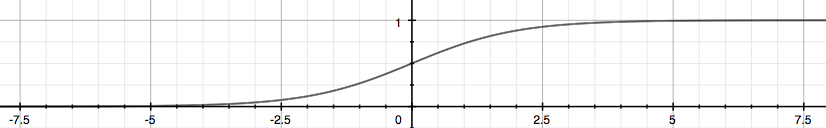
\includegraphics[scale=0.5]{W3_sigmoid}
\caption{Sigmoid Function}
\label{fig:W3_sigmoid}
\end{figure}

The function g(z), shown here, maps any real number to the (0, 1) interval, making it useful for transforming an arbitrary-valued function into a function better suited for classification. Try playing with interactive plot of sigmoid function: \href{https://www.desmos.com/calculator/bgontvxotm}{click here!}.

We start with our old hypothesis (linear regression), except that we want to restrict the range to 0 and 1. This is accomplished by plugging $\theta^T $ into the Logistic Function.

$h_\theta $ will give us the probability that our output is 1. For example, $h_\theta(x)=0.7$ gives us the probability of 70\% that our output is 1.

\begin{align*}
&h_\theta(x) = P(y=1 | x ; \theta) = 1 - P(y=0 | x ; \theta) \\ 
&P(y = 0 | x;\theta) + P(y = 1 | x ; \theta) = 1
\end{align*}

Our probability that our prediction is 0 is just the complement of our probability that it is 1 (e.g. if probability that it is 1 is 70\%, then the probability that it is 0 is 30\%).
\section{Decision Boundary}
In order to get our discrete 0 or 1 classification, we can translate the output of the hypothesis function as follows:
\begin{align*}
& h_\theta(x) \geq 0.5 \rightarrow y = 1 \\
& h_\theta(x) < 0.5 \rightarrow y = 0 \\
\end{align*}
The way our logistic function g behaves is that when its input is greater than or equal to zero, its output is greater than or equal to 0.5:
\begin{align*}
g(z) \geq 0.5 \\
\text{when } z \geq 0
\end{align*}
Remember:
\begin{align*}
z=0,  e^{0}=1 \Rightarrow  g(z)=1/2\\ 
z \to \infty, e^{-\infty} \to 0 \Rightarrow g(z)=1 \\ 
z \to -\infty, e^{\infty}\to \infty \Rightarrow g(z)=0 
\end{align*}

So if our input to g is $\theta^T$, then that means:
\begin{align*}
& h_\theta(x) = g(\theta^T x) \geq 0.5 \\
& \text{when} \; \theta^T x \geq 0
\end{align*}

From these statements we can now say:
\begin{align*}
& \theta^T x \geq 0 \Rightarrow y = 1 \\
& \theta^T x < 0 \Rightarrow y = 0 \\
\end{align*}

The {\bf decision boundary} is the line that separates the area where y = 0 and where y = 1. It is created by our hypothesis function.

Example:
\begin{align*}
& \theta = 
\begin{bmatrix}
5 \\ 
-1 \\ 
0
\end{bmatrix} \\ 
& y = 1 \; if \; 5 + (-1) x_1 + 0 x_2 \geq 0 \\ 
& 5 - x_1 \geq 0 \\ 
& - x_1 \geq -5 \\
& x_1 \leq 5 \\ 
\end{align*}

In this case, our decision boundary is a straight vertical line placed on the graph where $x_1 = 5$, and everything to the left of that denotes y = 1, while everything to the right denotes y = 0.

Again, the input to the sigmoid function g(z) (e.g. $\theta^T X$) doesn't need to be linear, and could be a function that describes a circle (e.g.$ z = \theta_0 + \theta_1 x_1^2 +\theta_2 x_2^2$) or any shape to fit our data.

\section{Cost Function}
We cannot use the same cost function that we use for linear regression because the Logistic Function will cause the output to be wavy, causing many local optima. In other words, it will not be a convex function.

Instead, our cost function for logistic regression looks like:
\begin{equation}
J(\theta) = \dfrac{1}{m} \sum_{i=1}^m \mathrm{Cost}(h_\theta(x^{(i)}),y^{(i)})
\end{equation}

\begin{align*}
\mathrm{Cost}(h_\theta(x),y) &= -\log(h_\theta(x)) \; \quad& \text{if y = 1} \\ 
\mathrm{Cost}(h_\theta(x),y) &= -\log(1-h_\theta(x)) \; \quad& \text{if y = 0}
\end{align*}

\begin{figure}[ht]
\center
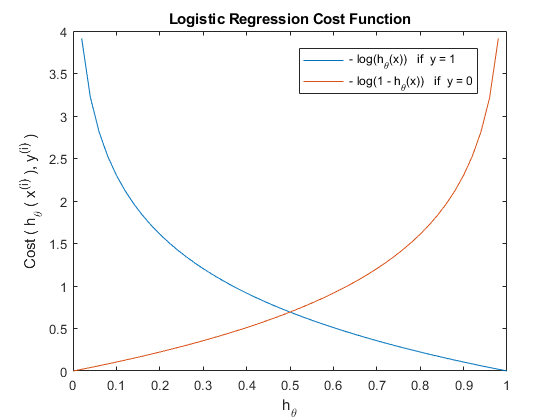
\includegraphics[scale=0.7]{W3_costlogistic}
\caption{Logistic Regression Cost Function}
\label{fig:W3_cost}
\end{figure}

The more our hypothesis is off from y, the larger the cost function output. If our hypothesis is equal to y, then our cost is 0:
\begin{align*}
& \mathrm{Cost}(h_\theta(x),y) = 0 \text{  if  } h_\theta(x) = y \\ 
& \mathrm{Cost}(h_\theta(x),y) \rightarrow \infty \text{  if  } y = 0 \; \mathrm{and} \; h_\theta(x) \rightarrow 1 \\ 
& \mathrm{Cost}(h_\theta(x),y) \rightarrow \infty \text{  if  } y = 1 \; \mathrm{and} \; h_\theta(x) \rightarrow 0 \\ 
\end{align*}
If our correct answer `y' is 0, then the cost function will be 0 if our hypothesis function also outputs 0. If our hypothesis approaches 1, then the cost function will approach infinity.

If our correct answer `y' is 1, then the cost function will be 0 if our hypothesis function outputs 1. If our hypothesis approaches 0, then the cost function will approach infinity.

Note that writing the cost function in this way guarantees that $J(\theta)$ is convex for logistic regression.

\section{Simplified Cost Function and Gradient Descent}
We can compress our cost function's two conditional cases into one case:

\begin{equation}
\mathrm{Cost}(h_\theta(x),y) = - y \; \log(h_\theta(x)) - (1 - y) \log(1 - h_\theta(x))
\end{equation}

Notice that when y is equal to 1, then the second term $(1-y)\log(1-h_\theta(x))$ will be zero and will not affect the result. If y is equal to 0, then the first term $-y \log(h_\theta(x))$ will be zero and will not affect the result.

We can fully write out our entire cost function as follows:

\begin{equation}
J(\theta) = - \frac{1}{m} \displaystyle \sum_{i=1}^m [y^{(i)}\log (h_\theta (x^{(i)})) + (1 - y^{(i)})\log (1 - h_\theta(x^{(i)}))]
\end{equation}

A vectorized implementation is:
\begin{align}
h &= g(X\theta)\\
J(\theta)  &= \frac{1}{m} \cdot \left(-y^{T}\log(h)-(1-y)^{T}\log(1-h)\right)
\end{align}

\subsection{Gradient Descent}
Remember that the general form of gradient descent is:
\begin{align*}
& Repeat \; \lbrace \\ 
& \; \theta_j := \theta_j - \alpha \dfrac{\partial}{\partial \theta_j}J(\theta) \\ 
& \rbrace
\end{align*}

We can work out the derivative part using calculus to get:

\begin{align*}
& Repeat \; \lbrace \\
& \; \theta_j := \theta_j - \frac{\alpha}{m} \sum_{i=1}^m (h_\theta(x^{(i)}) - y^{(i)}) x_j^{(i)} \\ & \rbrace
\end{align*}

Notice that this algorithm is identical to the one we used in linear regression. We still have to simultaneously update all values in theta.

A vectorized implementation is:
\[\theta := \theta - \frac{\alpha}{m} X^{T} (g(X \theta ) - \vec{y}) \]

\subsection{Partial derivative of Cost Function}

First calculate derivative of sigmoid function (it will be useful while finding partial derivative of $J(\theta)$

{\small
\begin{align*}
\sigma(x)'
&=\left(\frac{1}{1+e^{-x}}\right)'=\frac{-(1+e^{-x})'}{(1+e^{-x})^2}\\
&=\frac{-1'-(e^{-x})'}{(1+e^{-x})^2}=\frac{0-(-x)'(e^{-x})}{(1+e^{-x})^2}\\
&=\frac{-(-1)(e^{-x})}{(1+e^{-x})^2}=\frac{e^{-x}}{(1+e^{-x})^2} \\ 
&=\left(\frac{1}{1+e^{-x}}\right)\left(\frac{e^{-x}}{1+e^{-x}}\right)\\
&=\sigma(x)\left(\frac{+1-1 + e^{-x}}{1+e^{-x}}\right)\\
&=\sigma(x)\left(\frac{1 + e^{-x}}{1+e^{-x}} - \frac{1}{1+e^{-x}}\right)\\
&=\sigma(x)(1 - \sigma(x))
\end{align*}
}

Now we are ready to find out resulting partial derivative:
{\small
\begin{align*}
&\frac{\partial}{\partial \theta_j} J(\theta)= \\ 
&= \frac{\partial}{\partial \theta_j} \frac{-1}{m}\sum_{i=1}^m \left [ y^{(i)} log (h_\theta(x^{(i)})) + (1-y^{(i)}) log (1 - h_\theta(x^{(i)})) \right ] \\
&= - \frac{1}{m}\sum_{i=1}^m \left [     y^{(i)} \frac{\partial}{\partial \theta_j} log (h_\theta(x^{(i)}))   + (1-y^{(i)}) \frac{\partial}{\partial \theta_j} log (1 - h_\theta(x^{(i)}))\right ] \\
&= - \frac{1}{m}\sum_{i=1}^m \left [     \frac{y^{(i)} \frac{\partial}{\partial \theta_j} h_\theta(x^{(i)})}{h_\theta(x^{(i)})}   + \frac{(1-y^{(i)})\frac{\partial}{\partial \theta_j} (1 - h_\theta(x^{(i)}))}{1 - h_\theta(x^{(i)})}\right ] \\
&= - \frac{1}{m}\sum_{i=1}^m \left [     \frac{y^{(i)} \frac{\partial}{\partial \theta_j} \sigma(\theta^T x^{(i)})}{h_\theta(x^{(i)})}   + \frac{(1-y^{(i)})\frac{\partial}{\partial \theta_j} (1 - \sigma(\theta^T x^{(i)}))}{1 - h_\theta(x^{(i)})}\right ] \\
&= - \frac{1}{m}\sum_{i=1}^m \left [     \frac{y^{(i)} \sigma(\theta^T x^{(i)}) (1 - \sigma(\theta^T x^{(i)})) \frac{\partial}{\partial \theta_j} \theta^T x^{(i)}}{h_\theta(x^{(i)})}   + \frac{- (1-y^{(i)}) \sigma(\theta^T x^{(i)}) (1 - \sigma(\theta^T x^{(i)})) \frac{\partial}{\partial \theta_j} \theta^T x^{(i)}}{1 - h_\theta(x^{(i)})}\right ] \\
&= - \frac{1}{m}\sum_{i=1}^m \left [     \frac{y^{(i)} h_\theta(x^{(i)}) (1 - h_\theta(x^{(i)})) \frac{\partial}{\partial \theta_j} \theta^T x^{(i)}}{h_\theta(x^{(i)})}   - \frac{(1-y^{(i)}) h_\theta(x^{(i)}) (1 - h_\theta(x^{(i)})) \frac{\partial}{\partial \theta_j} \theta^T x^{(i)}}{1 - h_\theta(x^{(i)})}\right ] \\
&= - \frac{1}{m}\sum_{i=1}^m \left [     y^{(i)} (1 - h_\theta(x^{(i)})) x^{(i)}_j - (1-y^{(i)}) h_\theta(x^{(i)}) x^{(i)}_j\right ] \\
&= - \frac{1}{m}\sum_{i=1}^m \left [     y^{(i)} (1 - h_\theta(x^{(i)})) - (1-y^{(i)}) h_\theta(x^{(i)}) \right ] x^{(i)}_j \\
&= - \frac{1}{m}\sum_{i=1}^m \left [     y^{(i)} - y^{(i)} h_\theta(x^{(i)}) - h_\theta(x^{(i)}) + y^{(i)} h_\theta(x^{(i)}) \right ] x^{(i)}_j \\
&= - \frac{1}{m}\sum_{i=1}^m \left [ y^{(i)} - h_\theta(x^{(i)}) \right ] x^{(i)}_j  \\
&= \frac{1}{m}\sum_{i=1}^m \left [ h_\theta(x^{(i)}) - y^{(i)} \right ] x^{(i)}_j
\end{align*}
}

The vectorized version:
\begin{equation}
\nabla J(\theta) = \frac{1}{m} \cdot X^T \cdot \left(g\left(X\cdot\theta\right) - \vec{y}\right)
\end{equation}

\section{Advances Optimization}
\textbf{``Conjugate gradient"}, \textbf{``BFGS"}, and \textbf{``L-BFGS"} are more sophisticated, faster ways to optimize $\theta$ that can be used instead of gradient descent. A. Ng suggests not to write these more sophisticated algorithms yourself (unless you are an expert in numerical computing) but use the libraries instead, as they're already tested and highly optimized. Octave provides them.

We first need to provide a function that evaluates the following two functions for a given input value $\theta$:

\begin{align*}
J(\theta)\\
\frac{\partial}{\partial\theta_j}J(\theta)
\end{align*}

We can write a single function that returns both of these:

\begin{verbatim}
function [jVal, gradient] = costFunction(theta)
  jVal = [...code to compute J(theta)...];
  gradient = [...code to compute derivative of J(theta)...];
end
\end{verbatim}

Then we can use octave's \verb| fminunc()| optimization algorithm along with the \verb|optimset()| function that creates an object containing the options we want to send to \verb| fminunc()|. (Note: the value for MaxIter should be an integer, not a character string - errata in the video at 7:30)

\begin{verbatim}
options = optimset('GradObj', 'on', 'MaxIter', 100);
      initialTheta = zeros(2,1);
      [optTheta, functionVal, exitFlag] = fminunc(@costFunction, initialTheta, options);
\end{verbatim}

We give to the function \verb| fminunc()| our cost function, our initial vector of theta values, and the \textbf{options} object that we created beforehand.

\section{Multiclass Classification: One-vs-all}
Now we will approach the classification of data into more than two categories. Instead of $y = {0,1}$ we will expand our definition so that $y = {0,1...n}$.

In this case we divide our problem into n+1 (+1 because the index starts at 0) binary classification problems; in each one, we predict the probability that `y' is a member of one of our classes.

\begin{align*}
& y \in \lbrace0, 1 ... n\rbrace \\
& h_\theta^{(0)}(x) = P(y = 0 | x ; \theta) \\
& h_\theta^{(1)}(x) = P(y = 1 | x ; \theta) \\
& \cdots \\
& h_\theta^{(n)}(x) = P(y = n | x ; \theta) \\
& \mathrm{prediction} = \max_i( h_\theta ^{(i)}(x) )\\
\end{align*}

We are basically choosing one class and then lumping all the others into a single second class. We do this repeatedly, applying binary logistic regression to each case, and then use the hypothesis that returned the highest value as our prediction.

\section{ML: Regularization}
{\bf The Problem of Overfitting}
Regularization is designed to address the problem of overfitting.

High bias or underfitting is when the form of our hypothesis function h maps poorly to the trend of the data. It is usually caused by a function that is too simple or uses too few features. eg. if we take $h_\theta(x) = \theta_0 + \theta_1x_1 + \theta_2x_2$ then we are making an initial assumption that a linear model will fit the training data well and will be able to generalize but that may not be the case.

At the other extreme, overfitting or high variance is caused by a hypothesis function that fits the available data but does not generalize well to predict new data. It is usually caused by a complicated function that creates a lot of unnecessary curves and angles unrelated to the data.

This terminology is applied to both linear and logistic regression. There are two main options to address the issue of overfitting:

\begin{itemize}
  \item[1)] Reduce the number of features
  \begin{itemize}
  	\item[A)] Manually select which features to keep. 
  	\item[B)] Use a model selection algorithm (studied later in the course).
  \end{itemize}
  \item[2)] Regularization
  \begin{itemize}
  	\item[A)] Keep all the features, but reduce the parameters $\theta_j$
  	\item[B)] Regularization works well when we have a lot of slightly useful features.
  \end{itemize}  
\end{itemize}

\section{Cost Function}
f we have overfitting from our hypothesis function, we can reduce the weight that some of the terms in our function carry by increasing their cost.

Say we wanted to make the following function more quadratic:

$$\theta_0 + \theta_1x + \theta_2x^2 + \theta_3x^3 + \theta_4x^4$$

We'll want to eliminate the influence of $\theta_3x^3$ and $\theta_4x^4$. Without actually getting rid of these features or changing the form of our hypothesis, we can instead modify our \textbf{cost function}:
\begin{equation}
min_\theta\ \dfrac{1}{2m}\sum_{i=1}^m (h_\theta(x^{(i)}) - y^{(i)})^2 + 1000\cdot\theta_3^2 + 1000\cdot\theta_4^2
\end{equation}

We've added two extra terms at the end to inflate the cost of $\theta_3$ and $\theta_4$. Now, in order for the cost function to get close to zero, we will have to reduce the values of $\theta_3$ and $\theta_4$ to near zero. This will in turn greatly reduce the values of $\theta_3x^3$ and $\theta_4x^4$ in our hypothesis function.

We could also regularize all of our theta parameters in a single summation:

\begin{equation}
min_\theta\ \dfrac{1}{2m}\ \left[ \sum_{i=1}^m (h_\theta(x^{(i)}) - y^{(i)})^2 + \lambda\ \sum_{j=1}^n \theta_j^2 \right]
\end{equation}

The $\lambda$, or lambda, is \textbf{the regularization parameter}. It determines how much the costs of our theta parameters are inflated. You can visualize the effect of regularization in this \href{https://www.desmos.com/calculator/1hexc8ntqp}{interactive plot}

Using the above cost function with the extra summation, we can smooth the output of our hypothesis function to reduce overfitting. If lambda is chosen to be too large, it may smooth out the function too much and cause underfitting.

\section{Regularized Linear Regression}
We can apply regularization to both linear regression and logistic regression. We will approach linear regression first.

\subsection{Gradient Descent}
We will modify our gradient descent function to separate out $\theta_0$ from the rest of the parameters because we do not want to penalize $\theta_0$.
\begin{align*}
& \text{Repeat}\ \lbrace \\
& \ \ \ \ \theta_0 := \theta_0 - \alpha\ \frac{1}{m}\ \sum_{i=1}^m (h_\theta(x^{(i)}) - y^{(i)})x_0^{(i)} \\
& \ \ \ \ \theta_j := \theta_j - \alpha\ \left[ \left( \frac{1}{m}\ \sum_{i=1}^m (h_\theta(x^{(i)}) - y^{(i)})x_j^{(i)} \right) + \frac{\lambda}{m}\theta_j \right] &\ \ \ \ \ \ \ \ \ \ j \in \lbrace 1,2...n\rbrace\newline
& \rbrace
\end{align*}

The term $\frac{\lambda}{m}\theta_j$ performs our regularization.
With some manipulation our update rule can also be represented as:

\begin{equation}
\theta_j := \theta_j(1 - \alpha\frac{\lambda}{m}) - \alpha\frac{1}{m}\sum_{i=1}^m(h_\theta(x^{(i)}) - y^{(i)})x_j^{(i)}
\end{equation}

The first term in the above equation, $1 - \alpha\frac{\lambda}{m}$ will always be less than 1. Intuitively you can see it as reducing the value of $\theta_j$ by some amount on every update.

Notice that the second term is now exactly the same as it was before.

\subsection{Normal Equation}
Now let's approach regularization using the alternate method of the non-iterative normal equation.

To add in regularization, the equation is the same as our original, except that we add another term inside the parentheses:

\begin{align*}
& \theta = \left( X^TX + \lambda \cdot L \right)^{-1} X^Ty \\
& \text{where}\ \ L = 
\begin{bmatrix} 
0 & & & & \\ 
& 1 & & & \\ 
& & 1 & & \\ 
& & & \ddots & \\
& & & & 1 \\
\end{bmatrix}
\end{align*}

L is a matrix with 0 at the top left and 1's down the diagonal, with 0's everywhere else. It should have dimension $(n+1)\times(n+1)$. Intuitively, this is the identity matrix (though we are not including $x_0$), multiplied with a single real number $\lambda$.

Recall that if $m \leq n$, then $X^TX$ is non-invertible. However, when we add the term $\lambda \cdot L$, then $X^TX + \lambda \cdot L$ becomes invertible.
 
 \section{Regularized Logistic Regression}
 
\chapter{Week 4}
\section{ML: Neural Networks: Representation}
\subsection{Non-linear Hypothesis}
Performing linear regression with a complex set of data with many features is very unwieldy. Say you wanted to create a hypothesis from three (3) features that included all the quadratic terms:

\begin{align*}
&g(\theta_0 + \theta_1 x_1^2 + \theta_2x_1x_2+ \theta_3x_1x_3 \\
&+ \theta_4x_2^2 + \theta_5x_2x_3 \\
&+\theta_6x_3^2)
\end{align*}

That gives us 6 features. The exact way to calculate how many features for all polynomial terms is the combination function with repetition:

\href{http://www.mathsisfun.com/combinatorics/combinations-permutations.html}{Combinations and permutations} $\frac{(n+r-1)!}{r!(n-1)!}$.

In this case we are taking all two-element combinations of three features: $\frac{(3 + 2 - 1)!}{(2!\cdot (3-1)!)} = \frac{4!}{4} = 6 $.
(\textbf{Note}: you do not have to know these formulas, I just found helpful for understanding).

For 100 features, if we wanted to make the quadratic we would get $ \frac{(100 + 2 - 1)!}{(2\cdot (100-1)!)} = 5050 $ resulting new features.

We can approximate the growth of the number of new features we get with all quadratic terms with $\mathcal{O}(n^2/2)$. And if you wanted to include all cubic terms in your hypothesis, the features would grow asymptotically at $\mathcal{O}(n^3)$. These are very steep growths, so as the number of our features increase, the number of quadratic or cubic features increase very rapidly and becomes quickly impractical.

Example: let our training set be a collection of 50 x 50 pixel black-and-white photographs, and our goal will be to classify which ones are photos of cars. Our feature set size is then n = 2500 if we compare every pair of pixels.

Now let's say we need to make a quadratic hypothesis function. With quadratic features, our growth is $\mathcal{O}(n^2/2)$. So our total features will be about $2500^2 / 2 = 3125000 $, which is very impractical.

Neural networks offers an alternate way to perform machine learning when we have complex hypotheses with many features.

\section{Neurons and the Brain}

Neural networks are limited imitations of how our own brains work. They've had a big recent resurgence because of advances in computer hardware.

There is evidence that \textbf{the brain uses only one ``learning algorithm"} for all its different functions. Scientists have tried cutting (in an animal brain) the connection between the ears and the auditory cortex and rewiring the optical nerve with the auditory cortex to find that the auditory cortex literally learns to see.

This principle is called ``\textbf{neuroplasticity}" and has many examples and experimental evidence.

\section{Model Representation I}
Let's examine how we will represent a hypothesis function using neural networks.

At a very simple level, neurons are basically computational units that take input \textbf{dendrites} as electrical input (called ``\textbf{spikes}") that are channeled to outputs (\textbf{axons}).

In our model, our dendrites are like the input features $x_1\cdots x_n$, and the output is the result of our hypothesis function:

In this model our $x0$ input node is sometimes called the ``bias unit." It is always equal to 1.

In neural networks, we use the same logistic function as in classification: $\frac{1}{1 + e^{-\theta^Tx}} $. In neural networks however we sometimes call it a \textbf{sigmoid} (logistic) activation function.

Our ``theta" parameters are sometimes instead called \textbf{weights} in the neural networks model.

Visually, a simplistic representation looks like:
\[ [x_0x_1x_2]\rightarrow [\quad] \rightarrow h_\theta (x) \]

Our input nodes (layer 1) go into another node (layer 2), and are output as the hypothesis function.

The first layer is called the \textbf{input layer} and the final layer the \textbf{output layer}, which gives the final value computed on the hypothesis.

We can have intermediate layers of nodes between the input and output layers called the \textbf{hidden layer}.

We label these intermediate or \textbf{``hidden"} layer nodes $a^2_0 \cdots a^2_n $ and call them \textbf{activation units}.

\begin{align*}
& a_i^{(j)} = \text{``activation" of unit $i$ in layer $j$} \\
& \Theta^{(j)} = \text{matrix of weights controlling function mapping from layer $j$ to layer $j+1$}
\end{align*}

If we had one hidden layer, it would look visually something like:

\[ [x_0x_1x_2]\rightarrow [a_1^{(2)}a_2^{(2)}a_3^{(2)}] \rightarrow h_\theta (x) \]

The values for each \textbf{activation} nodes is obtained as follows:
\begin{align*}
a_1^{(2)} &= g(\Theta_{10}^{(1)}x_0 + \Theta_{11}^{(1)}x_1 + \Theta_{12}^{(1)}x_2 + \Theta_{13}^{(1)}x_3) \\
a_2^{(2)} &= g(\Theta_{20}^{(1)}x_0 + \Theta_{21}^{(1)}x_1 + \Theta_{22}^{(1)}x_2 + \Theta_{23}^{(1)}x_3) \\
a_3^{(2)} &= g(\Theta_{30}^{(1)}x_0 + \Theta_{31}^{(1)}x_1 + \Theta_{32}^{(1)}x_2 + \Theta_{33}^{(1)}x_3) \\ \\
h_\Theta(x) = a_1^{(3)} &= g(\Theta_{10}^{(2)}a_0^{(2)} + \Theta_{11}^{(2)}a_1^{(2)} + \Theta_{12}^{(2)}a_2^{(2)} + \Theta_{13}^{(2)}a_3^{(2)})
\end{align*}

This is saying that we compute our activation nodes by using a 3x4 matrix of parameters. We apply each row of the parameters to our inputs to obtain the value for one activation node. Our hypothesis output is the logistic function applied to the sum of the values of our activation nodes, which have been multiplied by yet another parameter matrix $\Theta^{(2)}$ containing the weights for our second layer of nodes.

Each layer gets its own matrix of weights, $\Theta^{(j)}$.

The dimensions of these matrices of weights is determined as follows:
\begin{quote}
If network has $s_j$ units in layer $j$  and $s_{j+1}$ units in layer $j+1$, then $\Theta_0^{j}$ will be of dimension $s_{s+j}\times(s_j+1)$
\end{quote}

The +1 comes from the addition in $\Theta^{(j)}$ of the \textbf{bias nodes}, $x_0$ and $\Theta_0^{(j)}$. In other words the output nodes will not include the bias nodes while the inputs will.

\textbf{Example}: layer 1 has 2 input nodes and layer 2 has 4 activation nodes. Dimension of $\Theta^{(1)}$ is going to be $4\times 3$ where $s_j = 2$ and $s_{j+1} = 4$, so: $$s_{j+1} \times (s_j + 1) = 4 \times 3$$

\section{Model Representation II}
In this section we'll do a vectorized implementation of the above functions. We're going to define a new variable $z_k^{(j)}$ that encompasses the parameters inside our g function. In our previous example if we replaced the variable z for all the parameters we would get:

\begin{align*}
a_1^{(2)} = g(z_1^{(2)}) \\
a_2^{(2)} = g(z_2^{(2)}) \\ 
a_3^{(2)} = g(z_3^{(2)})
\end{align*}
In other words, for layer j=2 and node k, the variable z will be:
\[
z_k^{(2)} = \Theta_{k,0}^{(1)}x_0 + \Theta_{k,1}^{(1)}x_1 + \cdots + \Theta_{k,n}^{(1)}x_n
\]

The vector representation of $x$ and $z^{j}$ is:
\begin{align*}
x = 
\begin{bmatrix}
x_0 \\ 
x_1 \\
\cdots \\ 
x_n
\end{bmatrix} 
&z^{(j)} = 
\begin{bmatrix}
z_1^{(j)} \\
z_2^{(j)} \\
\cdots \\ 
z_n^{(j)}
\end{bmatrix}
\end{align*}

Setting $x = a^{(1)}$, we can rewrite the equation as:

\[z^{(j)} = \Theta^{(j-1)} a^{(j-1)} \]

We are multiplying our matrix $\Theta^{(j-1)}$ with dimensions $s_j\times (n+1)$ (where $s_j$ is the number of our activation nodes) by our vector $a^{(j-1)}$ with height $(n+1)$. This gives us our vector $z^{(j)}$ with height $s_j$.

Now we can get a vector of our activation nodes for layer j as follows:

$$a^{(j)} = g(z^{(j)})$$

Where our function g can be applied element-wise to our vector $z^{(j)}$.

We can then add a bias unit (equal to 1) to layer j after we have computed $a^{(j)}$. This will be element $a_0^{(j)}$ and will be equal to 1.

To compute our final hypothesis, let's first compute another z vector:

$$ z^{(j+1)} = \Theta^{(j)}a^{(j)} $$


We get this final z vector by multiplying the next theta matrix after $\Theta^{(j-1)}$ with the values of all the activation nodes we just got.

This last theta matrix $\Theta^{(j)}$ will have only one row so that our result is a single number.

We then get our final result with:

\begin{equation}
h_\theta (x) = a^{(j+1)} = g(z^{(j+1)})
\end{equation}

Notice that in this \textbf{last step}, between layer j and layer j+1, we are doing \textbf{exactly the same thing} as we did in logistic regression.

Adding all these intermediate layers in neural networks allows us to more elegantly produce interesting and more complex non-linear hypotheses.
\section{Examples and Intuitions I}
A simple example of applying neural networks is by predicting $x_1$ AND $x_2$, which is the logical `\textbf{and}' operator and is only true if both $x_1$ and $x_2$ are 1.

The graph of our functions will look like:

\begin{align*}
\begin{bmatrix}
x_0 \\ 
x_1 \\ 
x_2
\end{bmatrix} 
\rightarrow
\begin{bmatrix}
g(z^{(2)})
\end{bmatrix} 
\rightarrow 
h_\Theta(x)
\end{align*}
Remember that $x_0$ is our bias variable and is always 1.

Let's set our first theta matrix as:

\begin{equation*}
\Theta^{(1)} = [-30\quad20\quad20]
\end{equation*}

This will cause the output of our hypothesis to only be positive if both $x_1$ and $x_2$ are 1. In other words:

\begin{align*}
& h_\Theta(x) = g(-30 + 20x_1 + 20x_2) \\ \\ 
& x_1 = 0 \ \ and \ \ x_2 = 0 \ \ then \ \ g(-30) \approx 0 \\ 
& x_1 = 0 \ \ and \ \ x_2 = 1 \ \ then \ \ g(-10) \approx 0 \\
& x_1 = 1 \ \ and \ \ x_2 = 0 \ \ then \ \ g(-10) \approx 0 \\ 
& x_1 = 1 \ \ and \ \ x_2 = 1 \ \ then \ \ g(10) \approx 1
\end{align*}
So we have constructed one of the fundamental operations in computers by using a small neural network rather than using an actual \textbf{AND} gate. Neural networks can also be used to simulate all the other logical gates.
\section{Examples and Intuitions II}
The $\Theta^{(1)}$ matrices for \textbf{AND}, \textbf{NOR} and \textbf{OR} are:
\begin{align*}
AND:\quad \Theta^{(1)} &= \begin{bmatrix}-30 & 20 & 20\end{bmatrix} \\ 
NOR:\quad \Theta^{(1)} &= \begin{bmatrix}10 & -20 & -20\end{bmatrix} \\
OR:\quad\Theta^{(1)} &= \begin{bmatrix}-10 & 20 & 20\end{bmatrix} \\
\end{align*}

We can combine these to get the \textbf{XNOR} logical operator (which gives 1 if $x_1x$ and $x_2$ are both 0 or both 1).
\begin{align*}
\begin{bmatrix}x_0 \\ 
x_1 \\ 
x_2
\end{bmatrix} 
\rightarrow
\begin{bmatrix}
a_1^{(2)} \\ 
a_2^{(2)} 
\end{bmatrix} 
\rightarrow
\begin{bmatrix}
a^{(3)}
\end{bmatrix} 
\rightarrow 
h_\Theta(x)
\end{align*}
For the transition between the first and second layer, we'll use a $\Theta^{(1)}$ matrix that combines the values for \textbf{AND} and \textbf{NOR}:
\begin{equation*}
\Theta^{(1)} = [-30\quad 20 \quad 2010 \quad -20 \quad -20]
\end{equation*}

For the transition between second and third layer, we'll use a $\Theta^{(2)}$ matrix that combines the values for \textbf{OR}:
\begin{equation*}
\Theta^{(1)} = [-30\quad 20 \quad 2010 \quad -20 \quad -20]
\end{equation*}

\begin{equation*}
\Theta^{(1)} = [-10\quad 20 \quad 20]
\end{equation*}

Let's write out the values for all our nodes:
\begin{align*}
& a^{(2)} = g(\Theta^{(1)} \cdot x) \\
& a^{(3)} = g(\Theta^{(2)} \cdot a^{(2)}) \\
& h_\Theta(x) = a^{(3)}
\end{align*}
\section{Multiclass Classification}

To classify data into multiple classes, we let our hypothesis function return a vector of values. Say we wanted to classify our data into one of four final resulting classes:

\begin{align*}
\begin{bmatrix} x_0 \\ x_1 \\ x_2 \\ \cdots \\ x_n \end{bmatrix} 
\rightarrow
\begin{bmatrix} a_0^{(2)} \\ a_1^{(2)} \\ a_2^{(2)} \\ \cdots \\ a_n^{(2)} \end{bmatrix} 
\rightarrow
\begin{bmatrix} a_0^{(3)} \\ a_1^{(3)} \\ a_2^{(3)} \\ \cdots \\ a_n^{(3)} \end{bmatrix} 
\rightarrow  \cdots \rightarrow
\begin{bmatrix} h_\Theta(x)_1 \\ h_\Theta(x)_2 \\ h_\Theta(x)_3 \\ h_\Theta(x)_4 \end{bmatrix} 
\rightarrow
\end{align*}

Our final layer of nodes, when multiplied by its theta matrix, will result in another vector, on which we will apply the g() logistic function to get a vector of hypothesis values.

Our resulting hypothesis for one set of inputs may look like:

$$
h_\Theta(x) = [0010]
$$

In which case our resulting class is the third one down, or $h_\Theta(x)_3$.

We can define our set of resulting classes as y:

\begin{equation*}
y^{(i)}= 
\begin{bmatrix}1\\0\\0\\0 \end{bmatrix},
\begin{bmatrix}0\\1\\0\\0 \end{bmatrix},
\begin{bmatrix}0\\0\\1\\0 \end{bmatrix},
\begin{bmatrix}0\\0\\0\\1 \end{bmatrix}
\end{equation*}

Our final value of our hypothesis for a set of inputs will be one of the elements in y.


\chapter{Week 5}
\section{Neural Networks Learning}
Let's first define a few variables that we will need to use:
\begin{itemize}
	\item[A)] L= total number of layers in the network
	\item[B)] $s_1$ number of units(not including bias unit) in layer 1
	\item[C)] K=number of outputs units/classes
\end{itemize}
Recall that the cost function for regularized logistic regression was:
\begin{equation}
J(\theta) = - \frac{1}{m} \sum_{i=1}^m \large[ y^{(i)}\ \log (h_\theta (x^{(i)})) + (1 - y^{(i)})\ \log (1 - h_\theta(x^{(i)}))\large] + \frac{\lambda}{2m}\sum_{j=1}^n \theta_j^2
\end{equation}
For neural  networks, it is going to bee slightly more complicated:

\section{The Problem of Overfitting}
Consider the problem of predicting y from $x \in R$. The leftmost figure \ref{fig:w3_overfit} shows the result of fitting a $y=\theta_0 + \theta_1 x$ to a dataset. We see that the data doesn't really lie on straight line, and so the fit is not very good.
\begin{figure}[ht]
\center
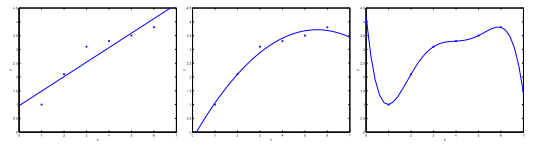
\includegraphics[scale=0.7]{W3_overfitting}
\caption{The Problem of Overfitting}
\label{fig:w3_overfit}
\end{figure}

Instead, if we had added an extra feature $x^2$, and fit $y = \theta_0 + \theta_1x + \theta_2x^2$, then we obtain a slightly better fit to the data (See middle figure). Naively, it might seem that the more features we add, the better. However, there is also a danger in adding too many features: The rightmost figure is the result of fitting a $5^{th}$ order polynomial $y = \sum_{j=0} ^5 \theta_j$. We see that even though the fitted curve passes through the data perfectly, we would not expect this to be a very good predictor of, say, housing prices (y) for different living areas (x). Without formally defining what these terms mean, we'll say the figure on the left shows an instance of {\bf underfitting}-in which the data clearly shows structure not captured by the model-and the figure on the right is an example of {\bf overfitting}.

Underfitting, or high bias, is when the form of our hypothesis function h maps poorly to the trend of the data. It is usually caused by a function that is too simple or uses too few features. At the other extreme, overfitting, or high variance, is caused by a hypothesis function that fits the available data but does not generalize well to predict new data. It is usually caused by a complicated function that creates a lot of unnecessary curves and angles unrelated to the data.

This terminology is applied to both linear and logistic regression. There are two main options to address the issue of overfitting:
\begin{itemize}
	\item[$1)$] Reduce the number of features:
	\item	\quad Manually select which features to keep.
	\item	\quad Use a model selection algorithm (studied later in the course).
	\item[$2)$] Regularization
	\item	\quad Keep all the features, but reduce the magnitude of parameters $\theta_j$
	\item	\quad Regularization works well when we have a lot of slightly useful features.
\end{itemize}
\newpage
\section{Summary}
\section*{Lineal Regression}
\subsection*{Hypothesis}
\begin{equation}
h_\theta (x) = \theta_0 + \theta_1 x_1 + \theta_2 x_2 + \theta_3 x_3 + \cdots + \theta_n x_n 
\end{equation}
\begin{align}
h_\theta(x) &= \theta^T x \\
h_\theta(X) &= X\theta 
\end{align}
\subsection*{Cost Function}
\begin{align}
J(\theta) &= \frac{1}{2m} \sum_{i=1}^m \left(h_\theta (x^{(i)}) - y^{(i)} \right)^2 \\
J(\theta) &= \frac{1}{2m} (X\theta - \vec{y})^T (X\theta - \vec{y})
\end{align}
\subsection*{Gradient Descent}
\begin{align}
\theta_j &:= \theta_j - \alpha \frac{1}{m} \sum\limits_{i=1}^{m} (h_\theta(x^{(i)}) - y^{(i)}) \cdot x_j^{(i)} \\
\theta &:= \theta - \frac{\alpha}{m}X^T (X\theta - \vec{y})
\end{align}
for j=0, 1,..., n:
\subsection*{Normal Equation}
\begin{equation}
\theta=(X^TX)^{-1}X^Ty
\end{equation}
\section*{Logistic Regression}
\subsection*{Hypothesis}
\begin{equation}
0 \leq h_\theta (x) \leq 1
\end{equation}
``Sigmoid Function," also called the ``Logistic Function":
\begin{align}
& h_\theta (x) =  g ( \theta^T x ) \\& z = \theta^T x \\& g(z) = \dfrac{1}{1 + e^{-z}}
\end{align}
\begin{align}
& h_\theta(x) = P(y=1 | x ; \theta) = 1 - P(y=0 | x ; \theta) \\& 
P(y = 0 | x;\theta) + P(y = 1 | x ; \theta) = 1
\end{align}
\subsection*{Cost Function}
\begin{equation}
J(\theta) = - \frac{1}{m} \displaystyle \sum_{i=1}^m [y^{(i)}\log (h_\theta (x^{(i)})) + (1 - y^{(i)})\log (1 - h_\theta(x^{(i)}))]
\end{equation}
\begin{align}
h &= g(X\theta)\\
J(\theta)  &= \frac{1}{m} \cdot \left(-y^{T}\log(h)-(1-y)^{T}\log(1-h)\right)
\end{align}
\subsection*{Gradient Descent}
\begin{align}
\theta_j &:= \theta_j - \frac{\alpha}{m} \sum_{i=1}^m (h_\theta(x^{(i)}) - y^{(i)}) x_j^{(i)} \\
\theta &:= \theta - \frac{\alpha}{m} X^{T} (g(X \theta ) - \vec{y})
\end{align}
\end{document}